\chapter{\label{ch:validation}Validation of the Simulation}
In order to validate our model, we had to compare the results obtained with our technique to another medically verified one. We chose the spirometer which is both the most widely used device and the \emph{de facto} standard pulmonary function testing device used by lung specialists. This chapter explains the technique used to test the validity of our method. Firstly, it describes the protocol followed to acquire data and provides an analysis of the data obtained on three subjects. Secondly, it states the different comparison techniques and the results achieved with our datasets.

% -------------------------------------------------------------
% Section
% -------------------------------------------------------------
\section{Experiment set up}
A laptop-based CardinalHealth UK MasterScope spirometer from Addenbrooke's hospital, Cambridge was kindly lent by Dr. Richard Iles, Consultant in Respiratory \& General Paediatrics, who is also involved in the SLP project. 
This system was chosen as it incorporates the widely used Fleish screen pneumotach. In addition, the derived flow signal can be exported in a machine-readable format using the manufacturers' software, JScope 32.

There are different techniques that can be used to design a spirometer; the one we used belongs to a specific type of spirometers called \emph{pneumotachometers}. A pneumotachometer measures the flow rate of gases by detecting pressure differences from a tube inserted in the mouth of the patient which is then processed to eventually give the volume flow over time. The pneumotachometer we used requires input of some of the patient's anatomy characteristics: gender, age, weight, height and the room conditions: altitude, humidity, pressure and temperature---this is probably used to correct the volume formulae applied by the device, though we have found very little detail in the technical documentation.

To compare our results to spirograms\footnote{A spirogram is a graph of respiratory movements from spirometry data.}, we performed both the SLP and spirometer measurements while subjects were breathing (see figure \ref{fig:tobi_resized}).

\begin{figure}
	\centering
	 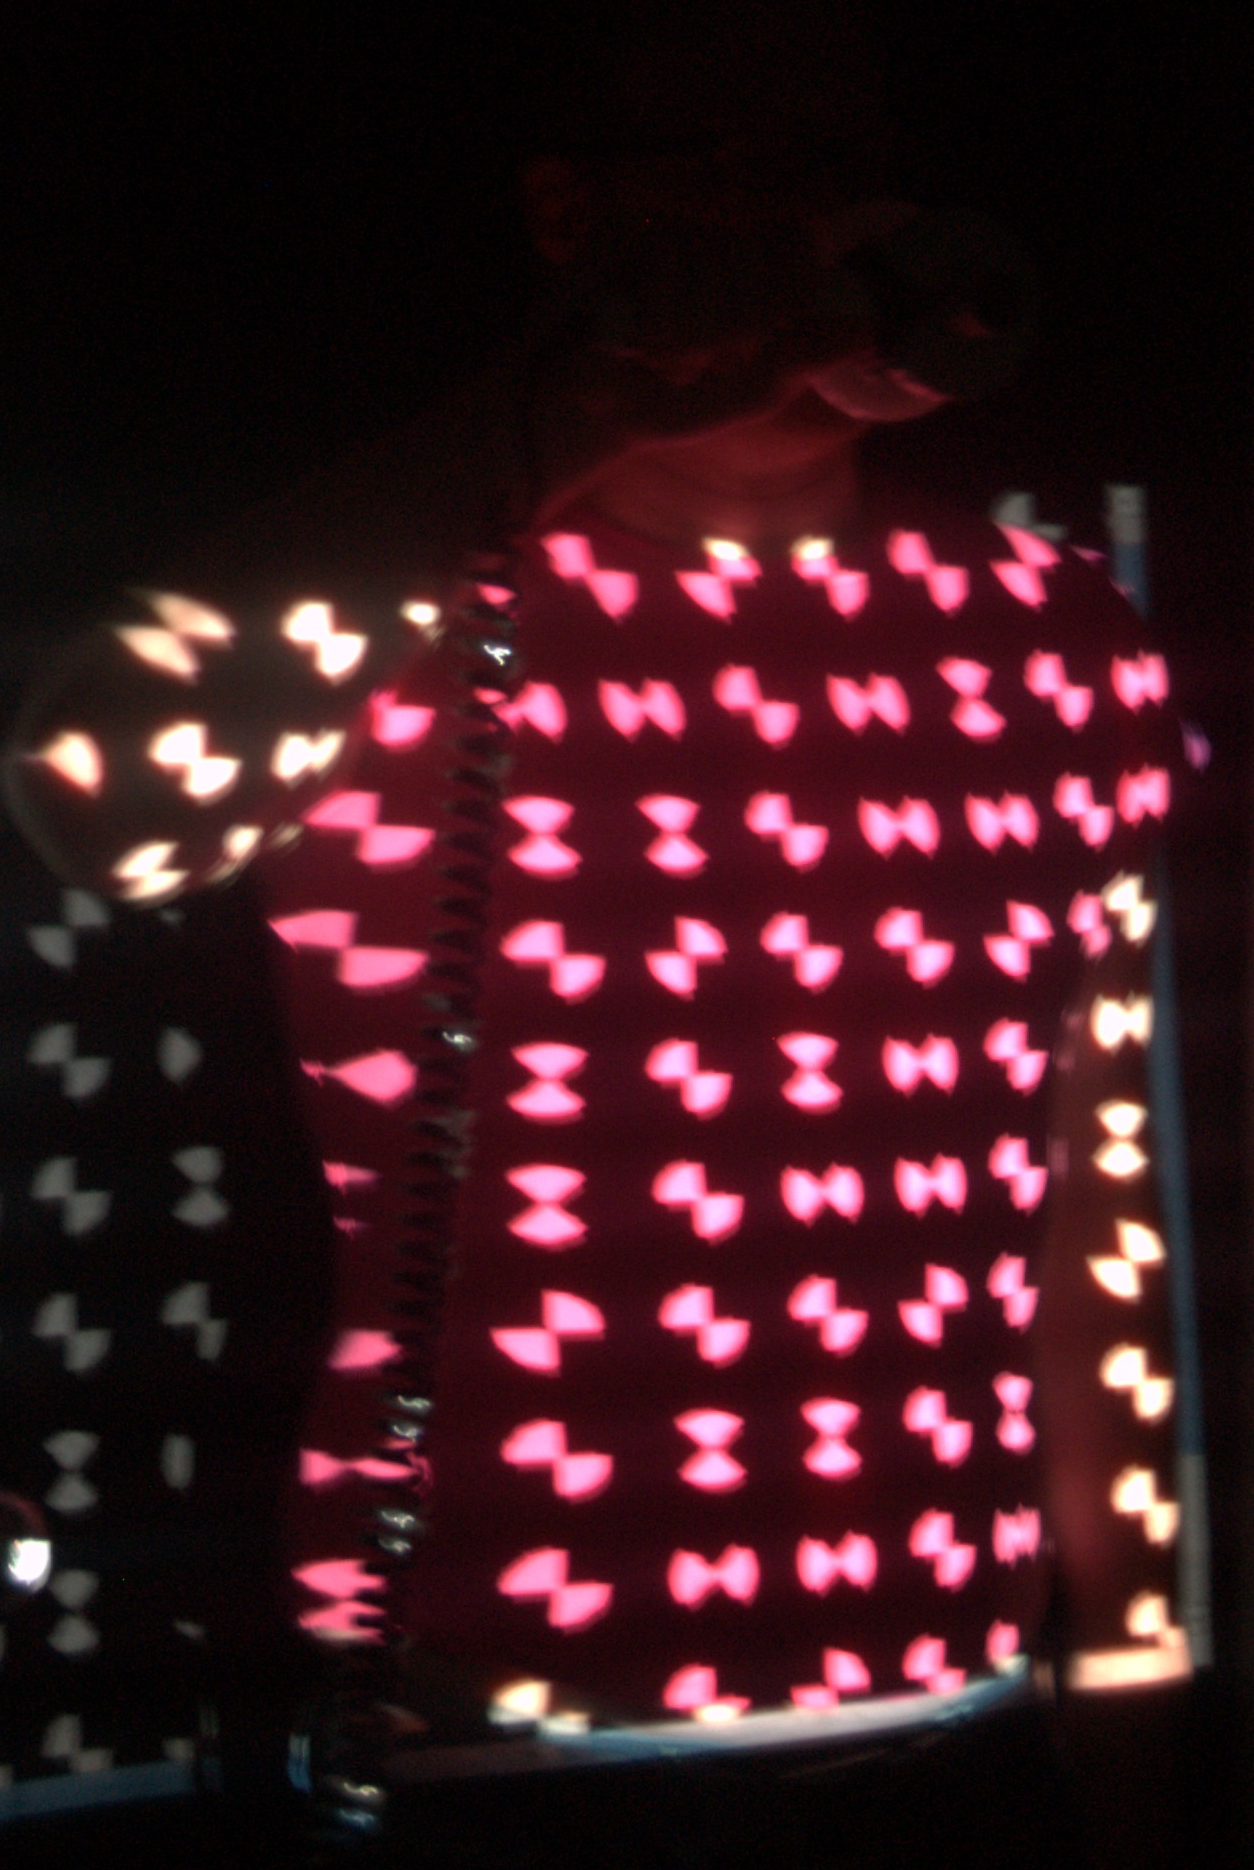
\includegraphics[width=0.5\textwidth]{pics/tobi_resized}
	\caption[Experiment set up]{\label{fig:tobi_resized}Experiment set up: both the SLP cameras and the spirometer are recording.}
\end{figure}

The validation of our technique was done by comparing estimations of the lung volume changes from the two different techniques on three male subjects of various anatomies (see table \ref{tab:patient_car}). 

After the system had made a zero flow calibration, the subject was asked to hold the spirometer head in the left hand, left elbow abducted so that the arm and cabling did not obstruct the camera image of the projected grid. He was then asked to start breathing in a relaxed and forced manner through the filter mouthpiece attachment in three different positions: standing, sitting and lying; this was done in order to assess the repeatability of the data collected under various conditions.

We deliberately asked the subjects to breathe in a regular tidal breathing fashion to reduce the optimisation time by decreasing the number of parameters to optimise over, while not compromising the validity of comparing the SLP and simulation results for validation purposes. Moreover, only the first 18 seconds (equivalent to 1000 samples as we normalise the data to 56~Hz) of the data were kept to reduce the computation of the cost function during the optimisation process.

\begin{table}
\begin{center}
\begin{tabular}{|c|c|c|c|c|c|}
\hline
subject & height (cm) & weight (kg) & age & BMI\footnotemark[1] & BSA\footnotemark[2] ($ m^2 $)\\ 
\hline
\hline
 1 & 175 & 65 & 23 & 21.2 & 1.79\\ 
 2 & 182 & 79 & 26 & 23.8 & 2\\ 
 3 & 180 & 92 & 33 & 28.4 & 2.12\\ 
\hline
\end{tabular}
\end{center}
\caption[Subjects's anatomy data]{\label{tab:patient_car}Subjects's anatomy data.}
\end{table}

\footnotetext[1]{Body Mass Index.}
\footnotetext[2]{Body Surface Area.}

% -------------------------------------------------------------
% Section
% -------------------------------------------------------------
\section{\label{sec:prep_data}Preparing the data for comparison}
The SLP system and pneumotach do not measure the same quantity and therefore direct comparisons are not possible. In order to make a meaningful comparison the SLP data and spirometry data have to be normalised.

SLP collects measurements at a rate of 56~Hz and so this is used as our simulation sample rate; on the other hand, spirometry operates at 100~Hz (see figures \ref{fig:prep_spir_ini} and \ref{fig:prep_simu_ini}). This means that while the curves represent data collected over the same period of time, the spirograms have 100/56 times more samples than the SLP data. Thus, we must re-sample and interpolate the spirometer data such that it is effectively sampled at a rate of 56~Hz. This is done in Matlab using the function \texttt{resample} (see figure \ref{fig:prep_spir_resampled}).

The simulation gives the volume changes of the thoracic cavity $V_{thoracic~cavity}(t)$, by subtracting the volume of the abdominal cavity from the total volume. Nevertheless, what the spirometer records is the volume flow of air at the exit of the mouth which is supposedly the volume flow of the lungs $V_{lungs}(t)$. Thus, what we need to compare to spirograms are the volume changes of the lungs from the simulation. As the lungs are contained within the thoracic cavity, their volumes are a ratio of the thoracic cavity (that could possibly vary from one patient to another, this will be discussed in section \ref{sec:bars}). To find this ratio, we used the \emph{3D Google Body anatomic model} \cite{googlebody2011} which is based on the data from Zygote Media Group 3D \cite{zygote2011}, and measured the different volumes of the big organs within the thoracic cavity (heart, ventricles, aorta, vena cava, esophagus) and the total volume of the cavity to deduce the ratio of the volume taken up by the lungs in this model. We found a ratio of 25~\%. Thus, we multiply the volume of the thoracic cavity given by our simulation by 75~\% to obtain the volume of the lungs to be compared to spirograms (see figure \ref{fig:prep_simu_lungs}).

Another issue that needs to be addressed is that the spirometry only measures the volume of air that is blown in and out from the mouth, which is in fact the volume flow of the lungs, whereas the simulation provides the variations of the absolute volume of the lungs. The consequence of this is that spirograms at time 0 start with a volume of value 0 and record the variations of air from this point, whereas the simulations at time 0, have a value that corresponds to the volume of the lungs at rest and give the variations of the volume of the lungs from this point.
To correct for this, we added the mean of the simulation data to the spirograms (see figure \ref{fig:prep_spir_mean}).

Finally, we must consider the fact that the SLP and spirometry data collection do not begin at precisely the same point in time as each technique is triggered manually and not synchronised at the beginning of the acquisition. To correct for this, we calculate the cross-correlations between the simulation data and the spirometry data over a lag of $\pm~100$ frames. We then find the lag which has the highest correlation, and adjust our data so that the highest correlation is at lag 0 (see figure \ref{fig:prep_simu_spir}). 

The different processed curves we obtained for each subject are available in appendix \ref{appendixA}.

\begin{figure}
\centering
\subfigure[]{
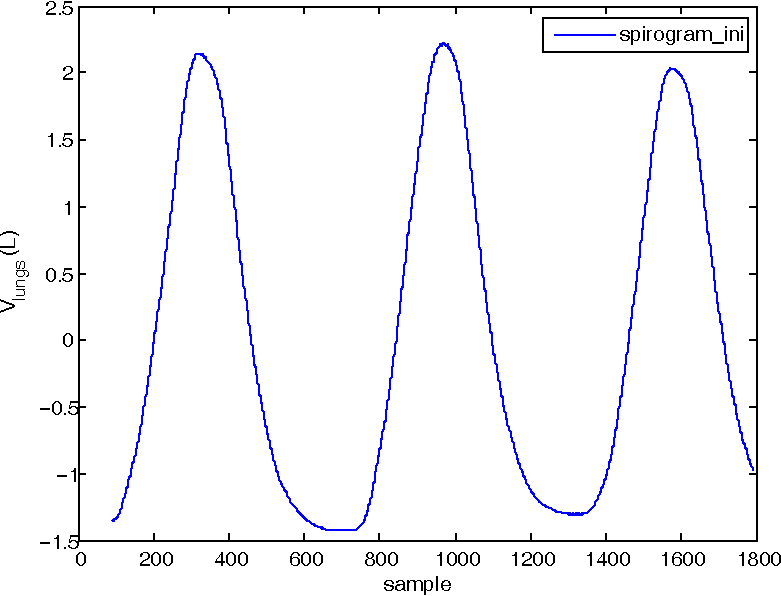
\includegraphics[width=0.47\textwidth]{pics/prep_spir_ini}
\label{fig:prep_spir_ini}
}
\subfigure[]{
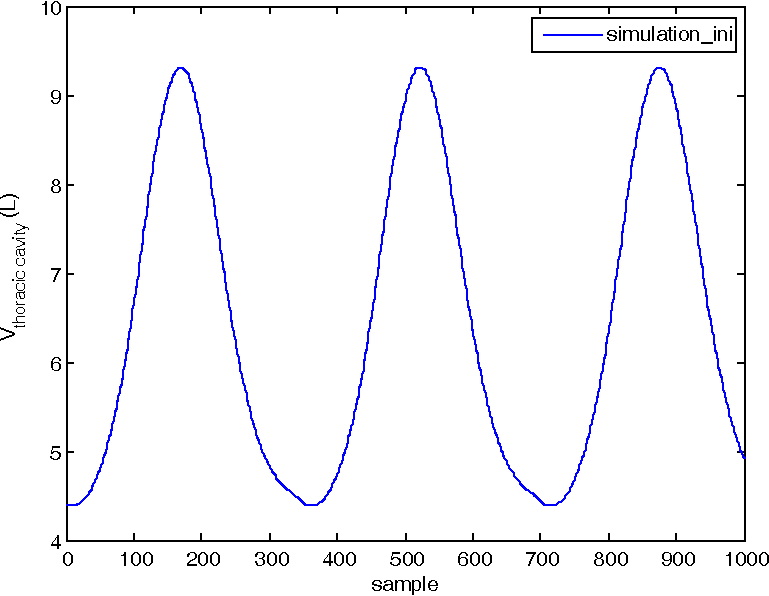
\includegraphics[width=0.47\textwidth]{pics/prep_simu_ini}
\label{fig:prep_simu_ini}
}
\subfigure[]{
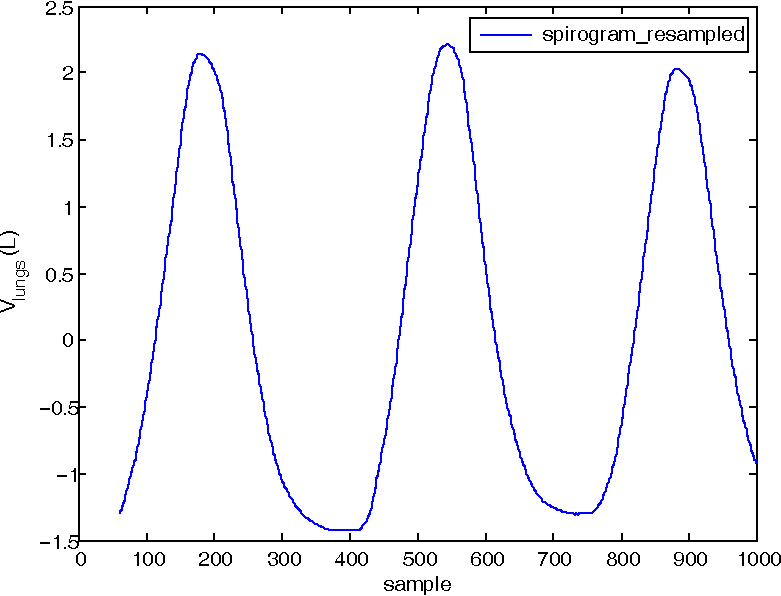
\includegraphics[width=0.47\textwidth]{pics/prep_spir_resampled}
\label{fig:prep_spir_resampled}
}
\subfigure[]{
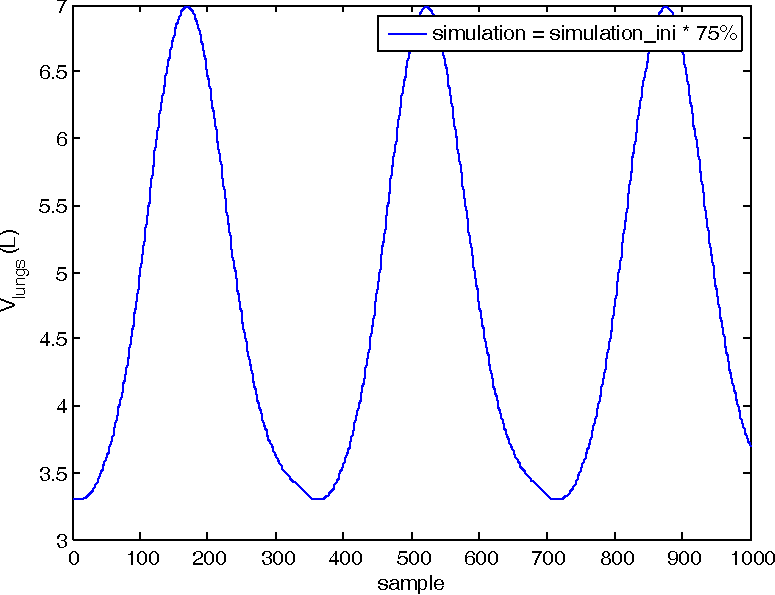
\includegraphics[width=0.47\textwidth]{pics/prep_simu_lungs}
\label{fig:prep_simu_lungs}
}
\subfigure[]{
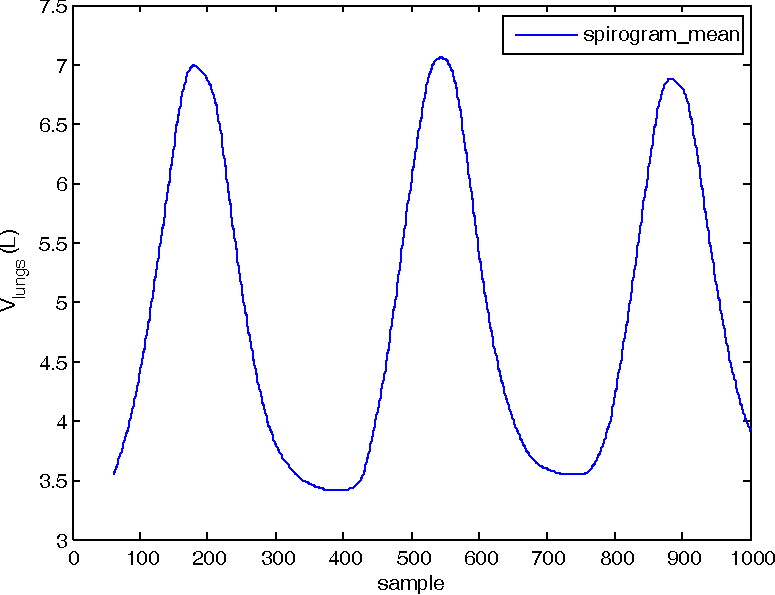
\includegraphics[width=0.47\textwidth]{pics/prep_spir_mean}
\label{fig:prep_spir_mean}
}
\subfigure[]{
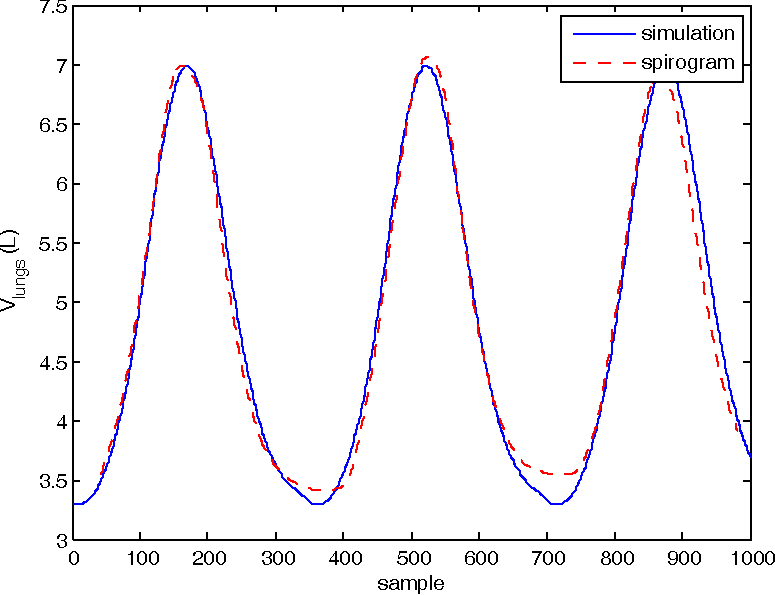
\includegraphics[width=0.47\textwidth]{pics/prep_simu_spir}
\label{fig:prep_simu_spir}
}
\caption[Preparation of the simulation and spirometry data before comparison]{\label{fig:preparing_spir_simu}Preparation of the simulation and spirometry data before comparison for (subject 1, standing, forced).
\subref{fig:prep_spir_ini} the raw spirometry and \subref{fig:prep_simu_ini} simulation curves have to be processed in order to compare them.
Firstly, \subref{fig:prep_spir_resampled} the spirogram has to be resampled at 56~Hz.
Secondly, \subref{fig:prep_simu_lungs} we take off 25~\% of the simulation volume curve to get the lung volume instead of the variations of the thoracic cage volume.
Thirdly, \subref{fig:prep_spir_mean} we add the mean of the simulation volume curve to the spirogram to get the absolute volume changes of the lungs.
Finally, \subref{fig:prep_simu_spir} we operate a cross-correlation algorithm to adjust the starting time of the simulation and spirometry curves.
}
\end{figure}

% -------------------------------------------------------------
% Section
% -------------------------------------------------------------
\section{\label{sec:optim_process}Optimisation process and data analysis}
The optimisation operates over the phases and magnitudes of the activations of the muscles of the rib cage and the abdomen. The breathing frequency $f_b$, is computed beforehand via a simple analysis of the fitting error over time; saving us one parameter to optimise over. We also assume that the activation functions are sine waves as they have been widely used in previous physically-based modelling of breathing work \cite{zordan2004breathe, lee2009comprehensive, veltkamp2009physiological} and have the great advantage of having few parameters to optimise over, which saves us considerable computational time. These assumptions will be questioned later on in this chapter.

\subsection{Performances of the optimisation}
The results of the first step which consists of fitting the skin mesh to the datasets are summarised in table \ref{tab:optim_res}. What we can infer from this is that the skin fitting process decreases the initial fitting error $FE_{ini}$, on average by $31~\%~\pm~6.5~\%$, leading to an average fitting error of $0.47~\mathrm{cm}~\pm~8.0~\%$ per grid point. 

In addition, the optimisation step gives satisfactory results for the average cost function values, $f_{error~optim}$ of $0.34~\mathrm{cm}~\pm~6.7~\%$ per grid point over the whole sequence. Only (subject 2, standing, forced) and (subject 3, lying, forced) cost function values were above 0.4~cm, which is slightly bigger than the others.
 
As we might expect, the fitting error is bigger for the forced breathing ($0.51~\mathrm{cm}~\pm~8.3~\%$) compared to the quiet breathing ($0.42~\mathrm{cm}~\pm~4.9~\%$), as the movements of both the thoracic and abdominal cavity are supposed to be larger; but interestingly enough, the cost function value for the forced breathing ($0.37~\mathrm{cm}~\pm~5.1~\%$) and the quiet breathing ($0.31~\mathrm{cm}~\pm~6.8~\%$) are both low and similar. This means, that the optimisation process does not do significantly worse when it comes to fitting larger breathing movements compared to calmer ones.

\begin{table}
\begin{center}
\begin{tabular}{|c|c|c|c|c|c|c|}
\hline
subject & position & breathing style & $FE_{init}$ & $FE_{fitted}$ & $f_{error~optim}$ & iterations\\ 
\hline
\hline

 \multirow{6}{*}{1} & \multirow{2}{*}{standing} & quiet & 0.6645 & 0.4230 & 0.3722 & 71\\ 
 & & forced & 0.7453 & 0.5286 & 0.3276 & 50\\ \cline{2-7}
 & \multirow{2}{*}{sitting} & quiet & 0.7402 & 0.3973 & 0.2679 & 63\\ 
 & & forced & 0.7947 & 0.5840 & 0.3617 & 56\\ \cline{2-7}
 & \multirow{2}{*}{lying} & quiet & 0.6108 & 0.4509 & 0.2567 & 68\\ 
 & & forced & 0.8562 & 0.6083 & 0.3894 & 47\\ \hline \hline
 
 \multirow{6}{*}{2} & \multirow{2}{*}{standing} & quiet & 0.5463 & 0.3369 & 0.2106 & 54\\ 
 & & forced & 0.6145 & 0.4972 & 0.4580 & 72\\ \cline{2-7}
 & \multirow{2}{*}{sitting} & quiet & 0.7393 & 0.4824 & 0.3505 & 50\\ 
 & & forced & 0.6533 & 0.4004 & 0.3725 & 66\\ \cline{2-7}
 & \multirow{2}{*}{lying} & quiet & 0.6207 & 0.4734 & 0.3836 & 68\\ 
 & & forced & 0.6612 & 0.4169 & 0.3216 & 61\\ \hline \hline
 
 \multirow{6}{*}{3} & \multirow{2}{*}{standing} & quiet & 0.5112 & 0.3665 & 0.2899 & 43\\ 
 & & forced & 0.8317 & 0.5927 & 0.3729 & 66\\ \cline{2-7}
 & \multirow{2}{*}{sitting} & quiet & 0.6198 & 0.4531 & 0.3913 & 57\\ 
 & & forced & 0.6067 & 0.4159 & 0.3105 & 68\\ \cline{2-7}
 & \multirow{2}{*}{lying} & quiet & 0.5705 & 0.4107 & 0.2427 & 45\\ 
 & & forced & 0.8585 & 0.5661 & 0.4427 & 71\\ 
 
\hline
\end{tabular}
\end{center}
\caption[Improvement provided by the skin fitting process over the skin error]{\label{tab:optim_res}Improvement provided by the skin fitting process over the skin error among different subjects breathing in different positions. The initial fitting error is given by $FE_{init}$ in cm, after fitting and smoothing the skin mesh as described in chapter \ref{ch:fitting_datasets} we obtain a new fitting error given by $FE_{fitted}$ (cm). $f_{error~optim}$ (cm) is the cost function value after optimisation, which is mathematically-wise the average of the fitting error when the skin mesh is deforming according to the optimised activations of the muscles over all the frames of the sequence.}
\end{table}

\subsection{Analysis of the optimisation outputs}
Table \ref{tab:optim_param} shows the exploitable outputs of the optimiser: the activation phases of the rib cage and abdomen ($\phi_{rc}$ and $\phi_{abd}$) and the activation ratios for the ribs and diaphragm, which are the ratios of the observed activations and the maximum reachable magnitudes of the rib muscles and diaphragm: $A_{ribs}$ and $A_{diaphragm}$ respectively.

\begin{table}
\begin{center}
\begin{tabular}{|c|c|c|c|c|c|c|}
\hline
 subject & position & breathing style & $\Delta_{\phi} = \phi_{abd} - \phi_{rc}$ & $A_{ribs}$ (\%) & $A_{diaphragm}$ (\%)\\ 
\hline
\hline

 \multirow{6}{*}{1} & \multirow{2}{*}{standing} & quiet & 0.21 & 23 & 26 \\ 
 & & forced & -0.051 & 37 & 41 \\ \cline{2-6}
 & \multirow{2}{*}{sitting} & quiet & 0.011 & 23 & 25 \\ 
 & & forced & -0.0031 & 38 & 42 \\ \cline{2-6}
 & \multirow{2}{*}{lying} & quiet & -0.39 & 8 & 48 \\ 
 & & forced & -0.2 & 35 & 51 \\ \hline \hline
 
 \multirow{6}{*}{2} & \multirow{2}{*}{standing} & quiet & 0.012 & 15 & 21 \\ 
 & & forced & 3.9 & 35 & 31 \\ \cline{2-6}
 & \multirow{2}{*}{sitting} & quiet & 0.16 & 12 & 20 \\ 
 & & forced & -1.4 & 28 & 23 \\ \cline{2-6}
 & \multirow{2}{*}{lying} & quiet & 0.013 & 3 & 12 \\ 
 & & forced & -0.053 & 23 & 25 \\ \hline \hline
 
 \multirow{6}{*}{3} & \multirow{2}{*}{standing} & quiet & 0.50 & 15 & 13  \\ 
 & & forced & -0.44 & 26 & 51 \\ \cline{2-6}
 & \multirow{2}{*}{sitting} & quiet & 0.071 & 25 & 31 \\ 
 & & forced & 1.6 & 31 & 49 \\ \cline{2-6}
 & \multirow{2}{*}{lying} & quiet & -0.051 & 2 & 8 \\ 
 & & forced & -0.32 & 12 & 32 \\
  
\hline
\end{tabular}
\end{center}
\caption[Optimal parameters found for the different datasets]{\label{tab:optim_param}Optimal parameters found for the different datasets. $\phi_{rc}$ and $\phi_{abd}$ are the activation phases of the rib cage and abdomen respectively. $A_{ribs}$ and $A_{diaphragm}$ correspond to the activation ratio of the maximum reachable magnitude of the rib muscles and the diaphragm respectively.
}
\end{table}

\subsubsection{Phase shift between the abdominal and rib cage cavities}
The absolute value of the phase shift $|\Delta_{\phi}| = |\phi_{abd} - \phi_{rc}|$ indicates how much the abdominal cavity and the rib cage movements are out of phase; its sign $sign(\Delta_{\phi})$, indicates which muscle group is fired first: if it is positive, the diaphragm is fired before the inspiratory muscles of the rib cage, otherwise it is the contrary.

We can make some observations on the results:
\begin{enumerate}
	\item During quiet breathing in 7/9 of the cases, $\Delta_{\phi} > 0$: the diaphragm is fired first. 
	\item During forced breathing in 7/9 of the cases, $\Delta_{\phi} < 0$: the rib cage is fired first.
	\item The value of the phase shift is bigger during quiet breathing than during forced breathing in 6/9 cases.
	\item The (subject 2, standing, forced) phase shift is nearly $\pi$ which tells that the diaphragm and the inspiratory muscles are nearly completely out of phase resulting in asynchronous breathing\footnote{Asynchronous breathing, also known as inverse breathing or paradoxical breathing, consists of expanding the abdomen while breathing out, and then compressing it while inhaling---the opposite of what an abdomen would do during natural breathing.} leading to poorer ventilatory mechanics which can cause serious respiratory illnesses.
\end{enumerate}

Points 1, 2 and 3 are \emph{en accord} with the study carried out by Sharp et al. \cite{sharp1975relative} on the relative contributions of rib cage and abdomen to breathing in normal subjects. According to \cite{sharp1975relative}, the rib cage is capable of more rapid contractions than the abdomen. As a consequence, for rapid manoeuvres such as forced breathing, intercostals and scalene muscles are called into action before the diaphragm; whereas during slow breathing, the diaphragm is nearly always fired before the rib cage muscles which is a trend we can observe in the results obtain.

Point 4 brings up an intriguing result as (subject 2, standing, forced) is not consistent with the other measurements taken from subject 2. If subject 2 had asynchronous breathing it would have affected all the measurements taken and subject 2 would not be in a healthy condition, as he indeed was. Looking more closely at the SLP data, we can definitely see an asynchronous breathing style in this specific position. The grid points of the SLP grid in the central part of the abdominal area are clearly out of phase compared to the grid points in the rib cage area. There were no obvious reasons for this abnormal breathing style except that subject 2 can willingly favour either his rib cage or abdomen to breathe and that while actively thinking about breathing normally in front of the SLP device, he might have produced an unnatural rather than an ordinary breathing style. More measurements on subject 2 were taken to test the reproducibility of the phenomenon, but we found no evidence of asynchronous breathing.

\subsubsection{Relative contributions from the abdominal and rib cage cavities}
$A_{ribs}$ and $A_{diaphragm}$ are the activation ratios of the observed activations to the maximum reachable magnitudes of the rib muscles and the diaphragm respectively found by the optimiser to fit the SLP data. They are an indication of the strength of the forces exerted by the muscles of the different cavities but cannot be compared to each other in terms of movement induced by the cavities on the external part of the body: having an $A_{ribs}$ of 40~\% and an $A_{diaphragm}$ of 60~\% does not necessarily mean that the motion of the abdominal area will be significantly bigger than the rib cage. In 15/18 of the cases in table \ref{tab:optim_param}, $A_{diaphragm}$ was bigger than $A_{ribs}$ which probably indicates one of two scenarios. The first is that all three subjects use the muscles of the diaphragm more than those of the rib cage. The second, and more likely, is that the result is simulation-dependent; the simulated diaphragm possibly needs a greater input to produce movement than the rib cage (which is linked to either the number of muscles used, the parameters of the different muscles, or the maximum value for the activation of the different muscles).

From the study detailed in \cite{sharp1975relative}, points of particular interest are:
\begin{enumerate}
	\item There are no major differences between men and women or between the young and the elderly during any respiratory acts.
	\item During quiet breathing most normal subjects are abdominal breathers when supine and thoracic breathers when upright (standing and sitting).
	\item Rapid manoeuvres are accomplished with a bigger contribution from the rib cage than from the abdomen.
	\item During forced breathing it appears that abdominal and rib cage muscles act to optimise the mechanical advantage of the diaphragm.	
\end{enumerate}

Considering the precautions we have to take concerning any comparison between $A_{ribs}$ and $A_{diaphragm}$ explained previously, we can however note that during quiet breathing in supine $A_{ribs}$ and $\frac{A_{ribs}}{A_{diaphragm}}$ have their lowest values than in any other position. This suggests first, that there is a smaller contribution from the rib cage while supine during quiet breathing than in any other position, secondly that the abdomen contributes significantly more than the rib cage in this configuration which is in accordance with point 2.

Concerning point 3, we can also see that the ratio $\frac{A_{ribs}}{A_{diaphragm}}$ during quiet breathing over all positions is on average $0.64~\pm~34~\%$ and $0.81~\pm~28~\%$ during forced breathing. What can be deduced from this is that the contribution of the rib cage compared to the abdomen during forced breathing is in proportion higher than during quiet breathing; which is precisely what point 3 highlights.  

% -------------------------------------------------------------
% Section
% -------------------------------------------------------------
\section{Comparing simulation and spirometry data}
Commonly, methods to assess agreements between two techniques of pulmonary function testing have relied on tools such as correlation coefficients, tests based upon pairing one's data and calculating the mean of the differences between the two methods, and the use of Bland-Altman plots to set a `limit of agreement' based on one's data.
This section will detail the results obtained with correlation coefficients and what can be inferred from them. Then, it will highlight the different specificities of Bland-Altman plots which are commonly used in medical statistics and the results obtained with this method. Finally, it will describe a frequentist and a Bayesian test on the null hypothesis that the two methods are equivalent for calculating tidal volumes, operating over both the raw time series data and the extracted parameters: the cosinor model and the BARS (Bayesian Adaptive Regression Splines) method. 

\subsection{\label{sec:corr_coeff}Correlation coefficient}
The most intuitive way to test whether or not two methods yield the same result is to compute the correlation between the results attained by the two techniques. The correlation coefficient $r$ is a statistic that measures the strength and the direction of a linear relationship between two variables. 

Table \ref{tab:likelihood} presents the correlation coefficients $r(sim,spir)$ between the simulation and spirometry data for each subject. Note that data for (subject 3, lying, quiet) is omitted; we see in figure \ref{appA:fig:p3} that the spirogram for this patient is abnormal (probably coming from bad handling of subject 3 during the measurement), as a consequence this dataset is not exploitable for comparison purposes and we did not compute the correlation coefficient, it will be omitted in what follows. The average correlation coefficient between the datasets---(subject 3, lying, quiet) omitted---is $0.88~\pm~5.8~\%$ which corresponds to a \emph{strong} correlation between the simulation and spirometry data.

Nonetheless, we have to bear in mind that the correlation coefficient has several flaws. First, it does not depend on the scale on which the data were collected and cannot be used in determining agreement between measurements when scale is of importance, as it is in our case (our main goal being finding the changes of the absolute volume of the lungs). Second, as explained by Bland and Altman \cite{altman1983measurement}, correlations depend solely on the variance between the true values and the variances of the methods, with low correlations potentially being obtained simply due to large amounts of noise within one's data. They also assert that correlation merely measures a relationship between the data and not an agreement.

The correlation coefficient method determines at a basic level that two methods are related. As a result, what we can reasonably infer from the high correlation coefficient values obtained, is that simulation and spirometry methods are related and give similar data. However, more refined methods have to been sought in order to validate our model.

\subsection{\label{sec:ba}The Bland-Altman plot}
The Bland-Altman plot is an analytical tool proposed by Bland and Altman \cite{altman1983measurement, martin1986statistical} to serve as a basic visual indicator of agreement between two methods. In fact, it is a plot of the difference between measurements using the two methods versus the average of the two measurements using both methods. Thus, a Bland-Altman plot provides a visual way to spot systematic errors. A dashed-dotted line for zero mean difference along with two dashed lines at $Mean_{diff}~\pm~1.96~\times~SD_{diff}$ are included in the plot. $Mean_{diff}$ is the mean of the difference between the two measurements, $\pm~1.96$ corresponds to the points in between which a $\mathcal{N}(0,1)$ distribution integrates to 0.95 defining the `limit of agreement' and $SD_{diff}$ is the standard deviation of the difference between the two measurements. Bland and Altman's assertion is that if the methods agree, then 95~\% of the points on said plot will fall within those confidence bounds.

The different Bland-Altman plots we obtained for each experiment are available in appendix \ref{appendixB}. Figures \ref{fig:ba_p1}, \subref{fig:ba_p2} and \subref{fig:ba_p3} present the Bland-Altman plots of all measurements for a single subject and figure \ref{fig:ba_tot} for the whole dataset. The Bland-Altman plots obtained present systematics due to the fact that the points in our data are causally correlated.

\begin{figure}
\centering
\subfigure[]{
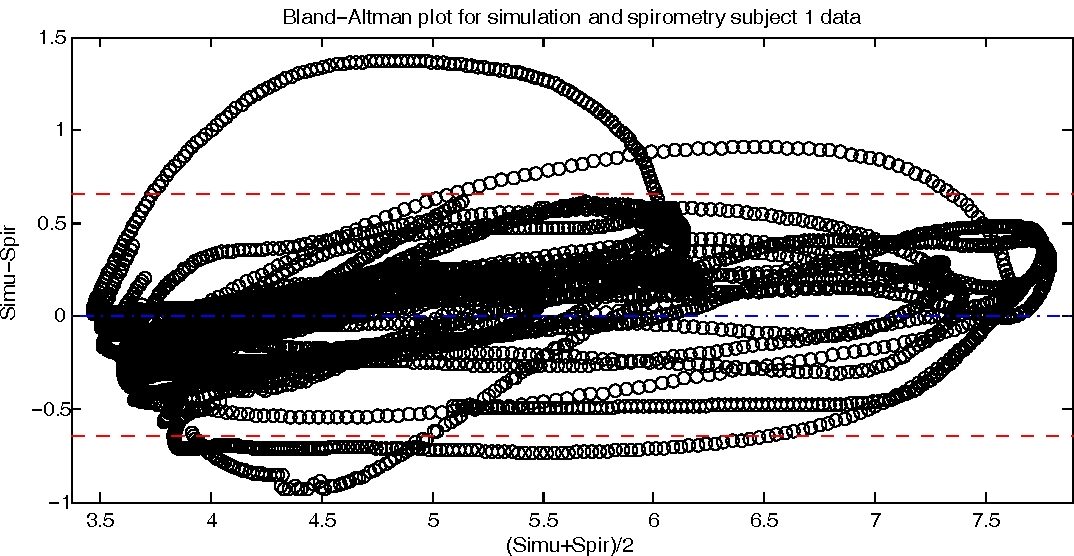
\includegraphics[width=0.475\textwidth]{pics/ba_p1}
\label{fig:ba_p1}
}
\subfigure[]{
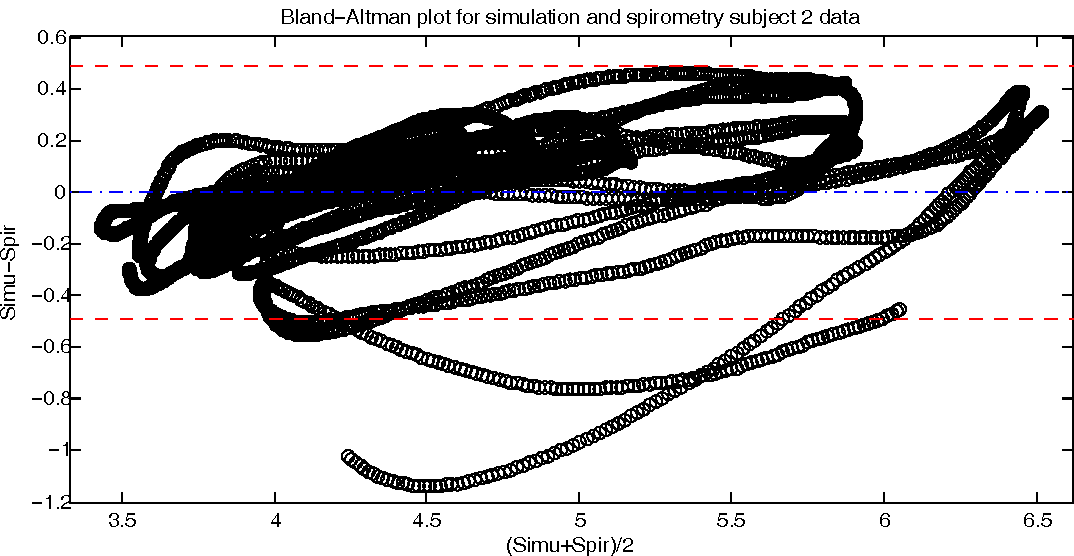
\includegraphics[width=0.475\textwidth]{pics/ba_p2}
\label{fig:ba_p2}
}
\subfigure[]{
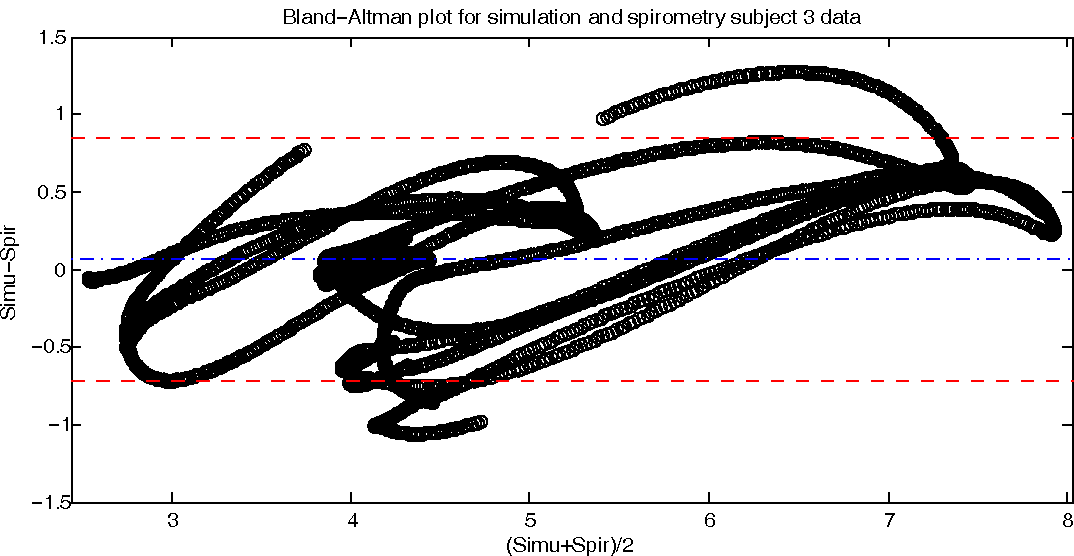
\includegraphics[width=0.475\textwidth]{pics/ba_p3}
\label{fig:ba_p3}
}
\subfigure[]{
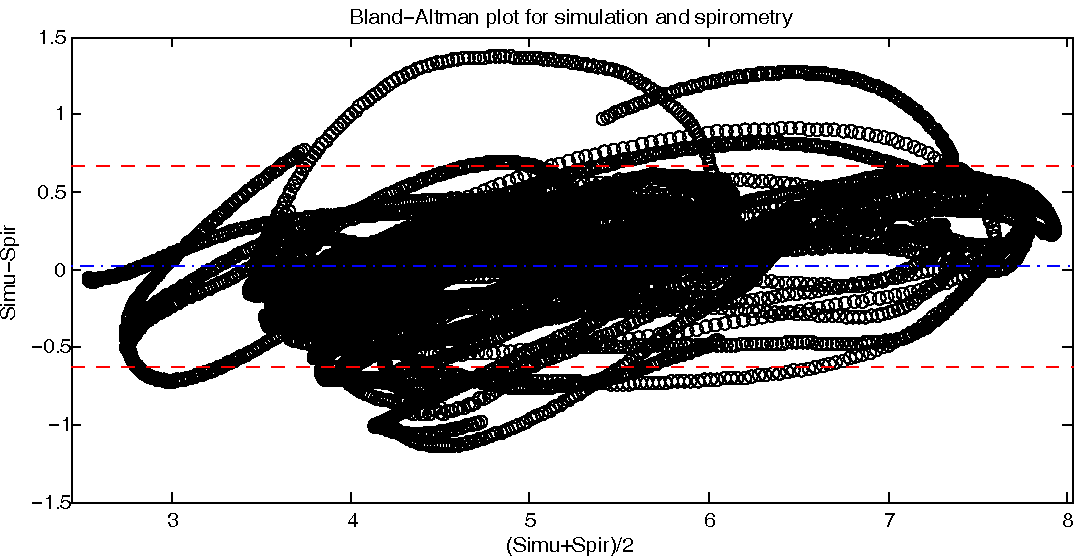
\includegraphics[width=0.475\textwidth]{pics/ba_tot}
\label{fig:ba_tot}
}

\caption[Bland-Altman plots for spirometry and simulation data]{\label{fig:ba_plots}Bland-Altman plots for spirometry and simulation data.
The blue dashed-dotted line corresponds to the zero mean difference and the red dashed lines to $\pm~1.96~\times~SD_{diff}$ from the mean in either direction defining the limits of agreement.
\subref{fig:ba_p1}, \subref{fig:ba_p2} and \subref{fig:ba_p3} are the Bland-Altman plots for all measurements for subjects 1, 2 and 3 respectively.
\subref{fig:ba_tot} is the Bland-Altman plot for the all data from all subjects.
}
\end{figure}

One can see that the Bland-Altman plots from our data give very good results with few points outside the Bland-Altman `limits of agreement', which is in keeping with the null hypothesis that the simulation and spirometry methods are the `same'. Thus, we can say that not only simulation and spirometry give similar results (as the correlation coefficient study showed in the previous section) but also that these two methods are measuring the `same' data (volume changes of the lungs). The question then arises as to whether the simulation and spirometry methods are {\textbf equal} and whether the Bland-Altman plots can provide an answer to this.
According to Fogarty \cite{fogarty2011slp}, the Bland-Altman plot is a useful reference for assessing equality between two methods, however it should only be considered as a visual aid or starting point in assessing strict equality between two methods. Moreover, Bland-Altman plots suffer from several flaws. For instance, the upper limits of the Bland-Altman plot will increase in range proportional to the magnitude of the variance. Thus, methods that vary from one another quite drastically but have an average difference of around 0 will seem perfectly acceptable based on the `limits of agreement'. To cope with the inherent flaws of Bland-Altman plots in assessing the {\textbf equality} between two methods, \cite{fogarty2011slp} derived testing techniques dealing with the underlying nature of the raw data from spirometry and SLP using the cosinor and BARS methods. These methods exploit the fact that rather than merely having one data point per subject, each collection of data results in a set of two time series, each containing hundreds of data points.

\subsection{The cosinor model}
The cosinor model presented by Nelson et al. \cite{nelson1979methods} is a way of utilising the known sinusoidal nature of a dataset and, given a set of known periodicities, fitting a series of cosine curves to the data using least squares regression. In fact, it fits the model according to the following relationship given in \cite{alberola2003simple}:

\begin{equation}
f(t)=M+\displaystyle\sum\limits_{i=1}^C A_{i} \mathrm{cos}(\omega_{i} t + \varphi_{i}) + \epsilon(t)
\end{equation}
 
where $M$ is an intercept coefficient, $A_{i}$ and $\varphi_{i}$ are coefficients to be estimated, $\omega_{i}$ are known frequencies obtained beforehand using a method such as Fast Fourier Transform, $\epsilon(t)$ is noise assumed to be IID $\mathcal{N}(0,\sigma^2)$ and $C$ is a user defined number of cosine curves to fit. For our purposes, we found that $C=4$ provided our fits with sufficiently accurate features while still maintaining parsimony.

For each cosine curve, we have two unknown parameters $A_{i}$ and $\varphi_{i}$ which must be calculated based upon the optimal fit to our data. We thus have a vector of parameters $\Theta=[M \; \beta_1 \; \gamma_1 \; \dotsc \; \beta_C \; \gamma_C]$, where $\beta_i = A_i \cos (\varphi_{i})$ and $\gamma_i = -A_i \sin (\varphi_{i})$, to estimate. For both the simulation and spirometry data, the vector of parameters $\Theta_{simu}$ and $\Theta_{spir}$ are estimated using a Multivariate Least Squares Regression. 

Figure \ref{fig:cos_fitting} shows a curve produced by the cosinor model to fit one of our simulation volume curves.

\begin{figure}
\centering

\subfigure[]{
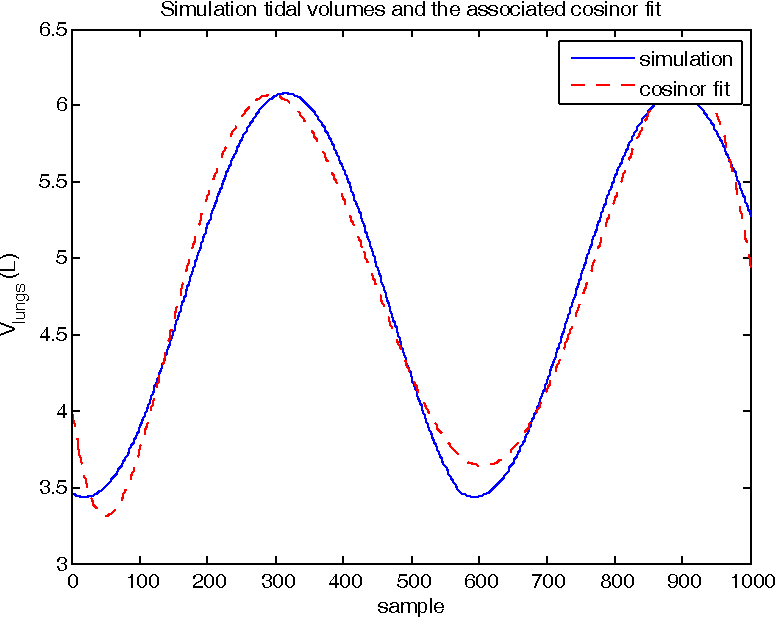
\includegraphics[width=0.475\textwidth]{pics/cos_simu}
\label{fig:cos_simu}
}
\subfigure[]{
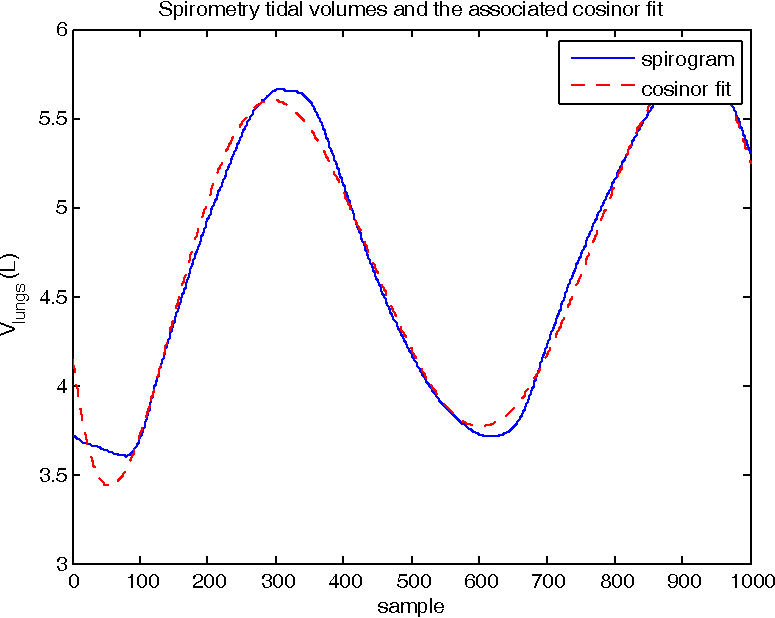
\includegraphics[width=0.475\textwidth]{pics/cos_spir}
\label{fig:cos_spir}
}

\caption[Simulation and spirometry data and the corresponding cosinor fits]{\label{fig:cos_fitting}Volume-time curves for \subref{fig:cos_simu} our simulation and \subref{fig:cos_spir} spirometry data (blue lines) and the corresponding cosinor fits (red dashed lines).
}
\end{figure}

The idea behind the cosinor model derived in \cite{fogarty2011slp} is to compare the parameter vectors to test the equality of the two methods assessed. \cite{fogarty2011slp} extends the cosinor model's derivation to a test of equality between two time series and adapts the said test to spirometry and SLP data.
Table \ref{tab:likelihood} reports the $p$-values associated with these tests for each of our datasets. The $p$-value serves as an indicator of evidence against our null hypothesis. \cite{fogarty2011slp} uses the standard threshold of $\alpha=0.05$ for determining if we can reject the null hypothesis that the coefficient vectors are the same. Furthermore, it has to be said that rather than finding out how likely it is that our null hypothesis is true, the frequentist hypothesis testing, which is at the heart of the cosinor method, calculates how unlikely a certain result is, given that our null hypothesis is true.
For an in depth description of assumptions and mathematics behind this technique, please consult the Master's thesis of Colin Fogarty \cite{fogarty2011slp}.

For our data collection, we find that of the 17 comparisons---(subject 3, lying, quiet) being omitted as justified in \ref{sec:corr_coeff}---, four of them ((subject 1 \& 3, standing, quiet), (subject 1, sitting, quiet) and (subject 3, lying, forced)) provide a $p$-value low enough to reject the null hypothesis. We will now investigate why these comparisons rejected the null hypothesis:

\begin{enumerate}
\item Looking at the simulation and spirometry curves for (subject 1, standing, quiet) in appendix \ref{appA:fig:p1}, we see that the spirogram at time $[150, 200]$ suffers from a variation that does not seem to be realistic and that could have appeared for many diverse reasons and also that there is a scale discrepancy. These facts led to a poor cosinor fit for the spirogram and thus would explain why the low $p$-value was obtained.

\item (Subject 1, sitting, quiet) does not appear to suffer from a poor cosinor fit. Comparing the curves more closely however, one can see that the spirogram and the simulation are slightly out of phase. This is due to the periodic nature of the activation inputs of the muscles. As explained in section \ref{sec:optim_process}, we optimised over sine function parameters as inputs to the respiratory muscles of the model to fit the SLP data, and worked on the assumption that the breathing style of each measurement was steady. As a consequence, the simulation data are periodic curves optimised to the SLP data. Although this is unlikely to be perfectly true all of the time, it is interesting to note that all other data is regular and periodic. As a consequence, we believe that the phase shift between the spirogram and the simulation curve was the main reason for the rejection of the null hypothesis in this case.

\item (Subject 3, standing, quiet) and (subject 3, lying, forced) show less conventional types of breathing. The shape of the spirograms can clearly be better described as a sawtooth shape rather than a sine wave shape (see \ref{appA:fig:p3}). Even though there are no obvious direct reasons that might explain this particular type of breathing, subject 3's general practitioner advanced the possibility that the \emph{polycystic kidney disease} that subject 3 has been suffering from, might explain this. A polycystic kidney disease is a cystic genetic disorder of the kidneys characterised by the presence of multiple cysts. The cysts are numerous and are fluid-filled, resulting in massive enlargement of the kidneys \cite{bisceglia2006renal}. This enlargement could possibly exert an extra pressure on the diaphragm and thus alter the breathing style. This breathing pattern has previously been seen in a number of people, who were not obviously suffering from any kidney disease. Nevertheless, this non-standard type of breathing is not perfectly reproduced by the simulation and this is clearly the reason why the null hypothesis was rejected for these datasets. It is important to note that the cosinor fitting to the spirograms was better in these cases than the others taken from subject 3 that have a `sawtooth'-like shape but which were not rejected. Looking at the spirogram more closely, the coefficient vector from the cosinor fit of the spirogram $\Theta_{spir}$ had more variable sine parameters which were not present in the coefficient vector of the cosinor fit of the simulation $\Theta_{simu}$. This could explain why the other curves did not fail to reject the null hypothesis (the coefficient vectors only having the core low variation sine parameters) and why these two rejected the null hypothesis.
 
\end{enumerate}
 
Thus, the reasons why these four datasets rejected the null hypothesis rely on either artefacts in data, non-periodic signals or non-conventional types of breathing, therefore pointing out limitations of the simulation technique. The factors that cause pairs to reject the null hypothesis according to the correlation and/or Bland-Altman studies are not obvious, but the cosinor model brings a better and more accurate understanding of the degree of similarity between data. 
From our data, we can see that the majority of our tidal volume curves fail to reject the null hypothesis that the two curves are the same. As a result, what we can say from the cosinor study is that the extracted cosine parameters from the simulation and the spirometry data are most of the time unlikely to be different. In other words, simulation and spirometry data coincide in their sinusoidal features.

However, as said previously, the frequentist approach provides no means of computing a concrete probability that one's null hypothesis actually is true, which is ultimately what a comparison study would like to show, but it is rather set up as a proof by contradiction.

\subsection{\label{sec:bars}BARS: Bayesian Adaptive Regression Splines}
Unlike the frequentist approach, the Bayesian paradigm attempts to calculate how likely the null hypothesis is. In our quest to test our null hypothesis that tidal volume curves produced by simulation and spirometry are the same, we now present an extension of a recently introduced method of curve fitting called Bayesian Adaptive Regression Splines (herein abbreviated as BARS) to give a test for equality of our two functions.

BARS is a Bayesian method for fitting curves to data based on a `signal plus noise' model developed by DiMatteo et al. \cite{dimatteo2001bayesian}, of the form:

\begin{equation}
y_j = f(x_j) + \epsilon_j
\end{equation}

This method uses B(asis)-Spline design matrices to fit splines of the third degree to data, and uses a reversible jump Metropolis-Hastings Markov Chain Monte Carlo simulation to select the location of the knots. The algorithm works by starting with an initial knot set specified by an uniform distribution on the location of these knots to be denoted as $\xi_{current}$, an initial number of knots $k_{current}$, and the resulting coefficient vector based on this knot set $\beta_{current}$, as well as a maximum number of knots that can be used in fitting the data. Then, with equal probability the algorithm decides to either generate a new knot, delete an existing knot or relocate a knot to a new position and thus creates a new knot set, number of knots and coefficient vector $\xi_{candidate}$, $k_{candidate}$ and $\beta_{candidate}$ respectively. Next the acceptance probability for the candidate knot set is calculated. If the acceptance probability $P(accept)$ is 1, then the new knot set is accepted making it the incumbent in subsequent runs of the MCMC. If it is $< 1$, then it accepts the new knot set with probability $P(accept)$. After running the simulation numerous times (for our data we do this 2000 times after an initial `burn-in' period of 200), we arrive at a B-spline design matrix that fits the data extremely well. Figure \ref{fig:bars_fitting} shows one of our tidal breathing sets with the corresponding fit produced by BARS using 10 knots overlaid.

\begin{figure}
\centering

\subfigure[]{
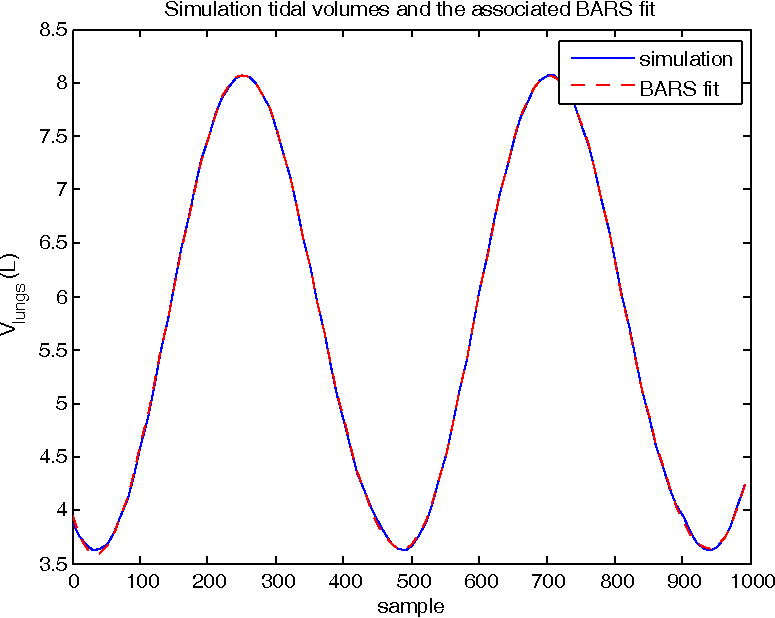
\includegraphics[width=0.475\textwidth]{pics/bars_simu}
\label{fig:bars_simu}
}
\subfigure[]{
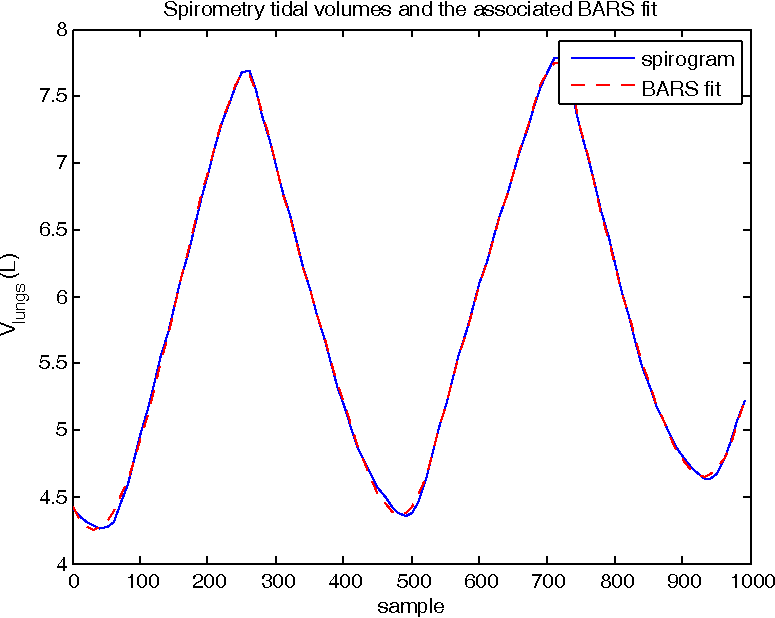
\includegraphics[width=0.475\textwidth]{pics/bars_spir}
\label{fig:bars_spir}
}

\caption[Simulation and spirometry data and the corresponding BARS fits]{\label{fig:bars_fitting}Volume-time curves for \subref{fig:bars_simu} our simulation and \subref{fig:bars_spir} spirometry data (blue lines) and the corresponding BARS fits (red dashed lines).
}
\end{figure}

Forgarty \cite{fogarty2011slp} then uses the method outlined by Behseta and Kass \cite{behseta2005testing}, which gives a means by which BARS can be modified such that it can be used to test equality of two curves in a Bayesian framework. Then he exploits the fact that BARS can simultaneously fit two curves and then compute the coefficient vector for fits of each dataset individually and for a fit of the two datasets simultaneously by restricting the curves to having the same knot set $\xi$. Based on this, he conducts a hypothesis test adapted to spirometry and SLP comparisons. The method tests whether the function that BARS fits to the first curve (simulation data) is the same as that fit to the second curve (spirometry data), by comparing how likely the joint fit of the two datasets is, relative to the likelihood of the fits of the two curves individually, with the constraint that the fits have used the same knot set. The null and alternative hypotheses being:

\begin{equation}
\begin{split}
\mathbf{H_o} : f_{spir}(t) = f_{simu}(t)
\\
\mathbf{H_a} : f_{spir}(t) \neq f_{simu}(t)
\end{split}
\end{equation}

The posterior probability $P(\mathbf{H_o} \mid simu,spir)$ of $\mathbf{H_o}$ is then computed based on the following:

\begin{equation}
P(\mathbf{H_o} \mid simu,spir) = \mathbb{E} \left[ P( \beta_{simu} = \beta_{spir} \mid \xi , simu, spir) \right]
\end{equation}

For the full details of the calculation and methodology, please refer to \cite{fogarty2011slp}.

Table \ref{tab:likelihood} shows our calculations of $P(\mathbf{H_o} \mid simu,spir)$ for our data. Looking at these values, we see that of the 17 pairs tested, two produced a strong probability (of 1 and 0.86) that the null hypothesis is true, 14 produced extremely low probabilities and the remaining one is in the middle giving a 0.18 probability. 
Comparing these probabilities to the cosinor $p$-values also displayed in \ref{tab:likelihood}, we see that the datasets which reject the null hypothesis for the cosinor model do not necessarily have low values of $P(\mathbf{H_o} \mid simu,spir)$ for our BARS comparison and vice-versa. For instance, (subject 2, standing, quiet) has a $p$-value of 0.95 which is the highest achieved in our dataset and an infinitesimal $P(\mathbf{H_o} \mid simu,spir)$ equal to $10^{-90}$. Conversely, (subject 1, standing, forced) gave a $P(\mathbf{H_o} \mid simu,spir)$ of 1 and a $p$-value of 0.57. This exemplifies the fact that the cosinor and the BARS methods do not assess the same features in comparing two datasets.

Our results tend to provide substantial evidence against our null hypothesis as very few comparison results were positive. From the BARS study we can deduce that the simulation and the spirometry do not provide the same data at a precise level. Several reasons could be explored to explain this conclusion:

\begin{enumerate}
	\item The BARS method tests the likelihood that two data are precisely the same and as such is very discriminative, whereas the cosinor tests the similarity of the data based on their frequency features---and we have seen that the simulation and the spirometry are very similar via the frequentist approach.  

	\item We made several assumptions for the optimisation process that can now be discussed. First, we used sine functions as inputs to the muscle activations, which is what has commonly been done in previous work on physically-based modelling \cite{zordan2004breathe, lee2009comprehensive, veltkamp2009physiological}. Even though the data obtained are very \textbf{similar} to spirometry as the correlation, Bland-Altman and cosinor studies showed, the results obtained with the BARS technique exposed that they are \textbf{not exactly the same} (the comparisons which rejected the cosinor tests were already indicating this fact). We believe that this is due to the true nature of the inputs. For instance, we tried to reproduce the sawtooth shape breathing of subject 3 by choosing different type of inputs and it seemed that deformed sine functions with a steeper slope in its ascending and descending part resulted in a simulated lung volume with a more `triangular' shape. One solution would be to optimise over a basis of functions as done in \cite{tu1994artificial}, but this is not currently feasible as it would require a huge increase in computational power. A less costly method worth investigation would be to optimise over periodic function parameters similar to sine; it would however inevitably introduce new parameters and significantly increase the optimisation time.
	
	\item Recall that one step in preparing the data for comparison is to take off 25~\% of the simulation curve to get the lung volume instead of the thoracic cage volume flow. This figure can possibly vary from one subject to another and affects the amplitude of the simulation data, which could result in poor agreement between the data and which would particularly affect the BARS method. To the best of our knowledge there are no non-invasive methods to accurately measure this figure.
\end{enumerate}

\begin{table}
\begin{center}
	
\begin{tabular}{|c|c|c|c|c|c|}
\hline
 subject & position & breathing style & $BARS(simu,spir)$ & $COS(simu,spir)$ & $r(simu,spir)$ \\ 
\hline
\hline

 \multirow{6}{*}{1} & \multirow{2}{*}{standing} & quiet & 0.18 & 0.035 & 0.78\\ 
 & & forced & 1 & 0.55 & 0.97 \\ \cline{2-6}
 & \multirow{2}{*}{sitting} & quiet & $10^{-11}$ & 0.0068 & 0.89\\ 
 & & forced & 0.86 & 0.57 & 0.91 \\ \cline{2-6}
 & \multirow{2}{*}{lying} & quiet & $10^{-107}$ & 0.71 & 0.94 \\ 
 & & forced & $10^{-100}$ & 0.11 & 0.97 \\ \hline \hline
 
 \multirow{6}{*}{2} & \multirow{2}{*}{standing} & quiet & $10^{-90}$ & 0.95 & 0.91 \\ 
 & & forced & $10^{-150}$ & 0.81 & 0.82 \\ \cline{2-6}
 & \multirow{2}{*}{sitting} & quiet & $10^{-116}$ & 0.91 & 0.91 \\ 
 & & forced & $10^{-42}$ & 0.62 & 0.95 \\ \cline{2-6}
 & \multirow{2}{*}{lying} & quiet & $10^{-108}$ & 0.060 & 0.87 \\ 
 & & forced & $10^{-146}$ & 0.23 & 0.91 \\ \hline \hline
 
 \multirow{6}{*}{3} & \multirow{2}{*}{standing} & quiet & $10^{-27}$ & 0 & 0.82 \\ 
 & & forced & $10^{-42}$ & 0.53 & 0.88 \\ \cline{2-6}
 & \multirow{2}{*}{sitting} & quiet & $10^{-75}$ & 0.44 & 0.81 \\ 
 & & forced & $10^{-89}$ & 0.088 & 0.82 \\ \cline{2-6}
 & \multirow{2}{*}{lying} & quiet & err & err & err \\ 
 & & forced & $10^{-66}$ & 0.021 & 0.86 \\

\hline
\end{tabular}
\end{center}
\caption[Results of the correlation, cosinor and BARS methods]{\label{tab:likelihood} 
The $BARS(simu,spir)$ column corresponds to $P(\mathbf{H_o} \mid simu,spir)$ which is the result of the BARS hypothesis test on the simulation and spirometry tidal volumes.
The $COS(simu,spir)$ column corresponds to the $p$-value of the cosinor method equality test between the simulation and spirometry data. 
The $r(simu,spir)$ column corresponds to the correlation coefficient between the simulation and spirometry data.
}
\end{table}